%% ---------------------------------------------------------------------
%% Copyright 2014, Thales, IGN, Rémi Cura
%% 
%% This file contains the introduction of article
%% ---------------------------------------------------------------------


\section{Introduction}

\begin{figure*}[t!]
	\begin{center}
		\fbox{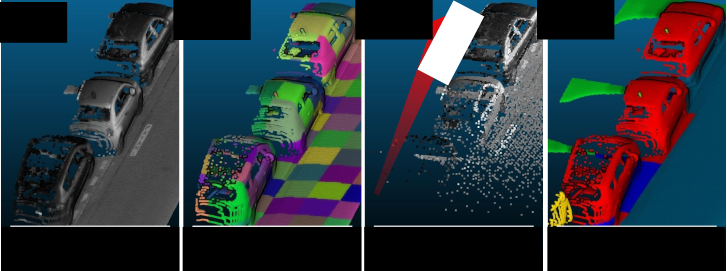
\includegraphics[width=\textwidth,keepaspectratio ]{./illustrations/banner_for_paper.png}}
		\caption{Data flow : a Lidar point cloud (1), is split it into patches (2) , patches are re-ordered to obtain free LOD (3 : a gradient of LOD here). Lastly the ordering is used as a feature for learning and efficient filtering (4) } 
		\label{fig:banner_image}
	\end{center}
\end{figure*} 

	\subsection{Problem}  
		Point cloud data is becoming more and more common. Following the same trend, the acquisition frequency and precision are also increasing.
		Thus point cloud processing is clocking on the Big Data door.
		
		Yet the usage of point cloud data is also spreading and going out of the traditional user communities. 
		Lidar are now commonly used by non-specialized users. 
		
		
		For many usage, having the raw, complete point cloud is unnecessary, or even damageable.
		Thus we deal with a simpler version of a problem that the G.I.S community has faced for a long time: how to generalize point cloud, with data sets that are several order of magnitude bigger than usual vector data set?
		
		It is after all a problematic very common in data processing. Having a big data set, how to reduce its size while preserving its characteristics.
		It is the essence of compression for instance.
		
		Generalization is also more difficult when mixing data set with varying densities. For instance an aerial Lidar map augmented at certain places by terrestrial scanners, or vehicle-based Lidar acquisition, where the density varies with speed and scene geometry. The illustration \ref{fig:hist-density-dataset} } shows the density variation in the two data set used for experiments in this article.
		
		Here we deal with a simplified version: given a point cloud, how to efficiently generate Level Of Detail (LOD, cf \href{banner_image}{figure ~\ref{fig:banner_image}}) of this point cloud while preserving the geometric characteristic, without duplicating data?
		The key to LOD approach is efficiency. Indeed LOD approaches sacrifices of a part of information in exchange of a massive reduction of data size. That's why a solution using LOD must by nature be efficient, or the information loss would be pointless.
		
	%	\paragraph{}
	\subsection{Motivation}
		\begin{itemize}
			\item Point cloud are becoming common. 
				Point cloud are becoming common because sensors are smaller, cheaper, easier to use. Point cloud from image (using Stereo Vision) are also easy to get with several mature structure from motion solutions.
				Point cloud complements very well images, Lidar point cloud allowing to avoid the ill-posed problem of stereo-vision, and providing key data to virtual reality.
			\item Growing data set and multi sources.
				At such the size of data set are growing, as well as the number of dataset and their diversity.
			\item A now widely use data type.
				The point cloud data are now well established in a number of industries, like construction, architecture, robotics, archaeology, as well as all the traditional GIS fields (mapping, survey, cultural heritage).
			\item Much less focus on informatics/storing.
				The LIDAR research community is very active. The focus of Lidar researchers is much more on Lidar processing and Lidar data analysis, or the sensing device, than on methods to render the data size tractable. 
		\end{itemize}   
		
	\subsection{State of the Art} 
		
		One way to tackle data size is to use a Level Of Detail strategy. Octree methods have been common in computer graphics for several decades \citep{Meagher1982}. They are used in many methods to speed computing, or compress data, like in the work of \cite{Schnabel2006,Huang2006} (which have not been designed to scale).
		
		\cite{Elseberg2013} give a good overview of octree usage for point clouds. Their method proposes to directly store the points and octree in a file. They explore many applications that could benefit from our method (visual LOD, registration, processing). We share many objectives. It is an extremely effective approach that also enables visual LOD, but is very specialized on geometry. In particular, this method is not integrated with other GIS data (Geographical Information System), point cloud fast querying is not possible on attributes or metadata, and point cloud format is extremely specific.
		\\
		Another orthogonal way is to use no file, but store point cloud in DBMS.  \cite{vanOosterom2014} implements such system at very big scale and discuss how it can answer to various need. This approach has gained recent interest \citep{pgPointCloud2014} because it is generic, it scales naturally to very large data set and is easier to implement than starting from scratch. We also observe that most of Big Data system use methods from the DBMS world.
		\\ 
		\cite{Demantke2014} introduces a sophisticated per-point dimensionality descriptor, which is used to find optimal neighbourhood size. A main difference is that this feature is computed for each point (thus is extremely costly to compute), and that dimensionality is influenced by density variation.
		
		Random Forest method started with \cite{Amit97shapequantization} and theorized by \cite{Breiman2001} and has been very popular since then. They are for instance used by \cite{Golovinskiy2009} who perform object detection, segmentation and classification. They analyse separately each task on an urban data set, thus providing valuable comparison. Their method is uniquely dedicated to this task, like \cite{Serna2014} who provide another method and a state of the art of the segmentation/classification subject.
		Both of this methods are in fact 2D methods, working on an elevation image obtained by projecting the point cloud. However we observe that street point clouds are dominated by vertical surfaces, like building (about 70\% in Paris data set). Our method is fully 3D and can then easily be used to detect vertical object details, like windows or doors on buildings.
		 
	
	\subsection{Contribution}
		This paper re-uses and combines existing and well established methods with a focus on simplicity and efficiency. As such, all the methods are tested on billions scale point cloud, and are Open Source for sake of reproducibility test and improvements.
		We propose a simple method that enables portable, computation-free, geometrical Level Of Detail.
		Our first contribution is to propose to store the LOD information directly into the ordering of points rather than externally, avoiding any data duplication.
		Thus, the more we read points, the more precise of an approximation of the point cloud we get. If we read all the points, we have the original point cloud.
		
		The second contribution is a simple way to order points in order to have an increasingly better geometric approximation of the point cloud when following this order.
		
		The third contribution is to use the ordering construction by-product as a simple and free dimensionality descriptor. We demonstrate the interest of this descriptor by performing a Random Forest classification that can then be used for very fast pre-filtering of points, and other applications.
			
		
	\subsection{Plan of the article}
		The rest of this article is organized as follows:
		in the next section \ref{sec:method} we present the methods.  
		In the result section \ref{sec:result} we give the results.
		We discuss it and the possible limitations in section \ref{sec:discussion}. 
